\chapter{Penetration Test Software and Tools}

Tools and Software used to execute a penetration test are the topics to be discussed in the following chapter. Penetration tester's tools are crucial elements to the outcome of the test. Proper selection of tools is done after thorough research on what each tool has to offer and which of those fit the needs and goals of the specific test to be performed. The main focus is to investigate the features provided by specific and well-known tools and operating systems and a comparison of those in order to decide upon the tools and their specifications that correspond to the test's architecture and goals. 

\section{Operating System Distributions}

Following, you will find a preview of some of the most well-known and widely used Penetration Testing operating systems. The focus is on open-source Linux distributions.

\begin{description}
\item[BackBox] Linux is a penetration testing and security assessment oriented Ubuntu-based distribution providing a network and systems analysis toolkit. Two of its most important features are \cite{arch2019doc}:
\begin{itemize}
\item[]
\textit{RAM Wiping} at shutdown/reboot keeps your system safe against attacks and make sure that nobody could compromise your privacy
\item[]
\textit{Full Hard Disk Encryption} in the installation phase by using LUKS\footnote{LUKS is the standard for Linux hard disk encryption. See more at \href{https://gitlab.com/cryptsetup/cryptsetup/blob/master/README.md}{their repositories}} on Local Volume Manager.
\end{itemize}
As a fast, easy to use, and efficient operating system, Backbox Linux is famous in the hacking community. The OS includes a complete desktop environment with software applications that are updated on a regular basis. 

\begin{figure}[H]
\centering
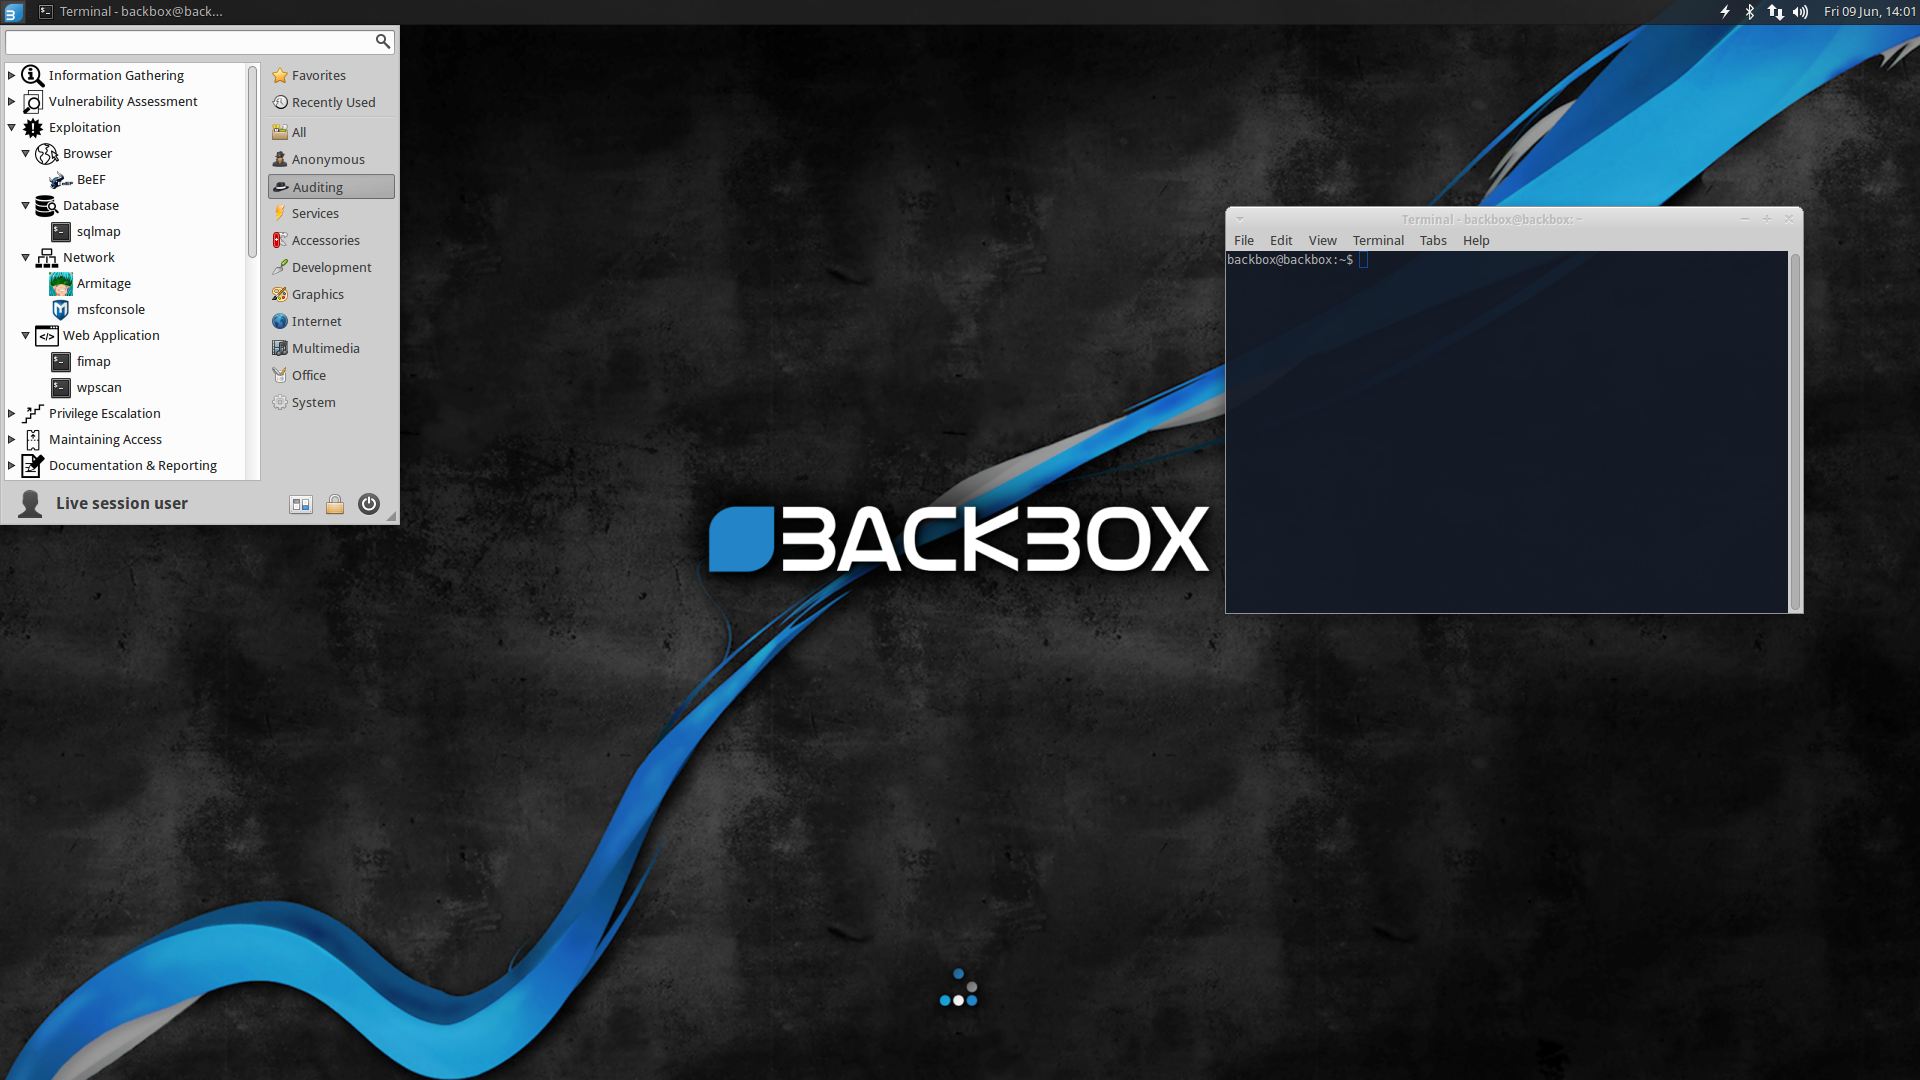
\includegraphics[width=1.0\textwidth]{Resources/Tools/BackBox.png}
\caption{BackBox Linux Desktop Environment}
\end{figure}

The interface is designed with the goal of minimalism, and utilizes a XFCE\footnote{Xfce is a lightweight desktop environment for UNIX-like operating systems. For more information, visit \href{https://xfce.org/about}{XFCE's website}} environment for its desktop. The result is an effective, fast, customizable, comprehensive user experience with a helpful support community to back it.
\bigskip

\item[BlackArch] Linux is a penetration testing specific design which originally derived from Arch Linux, and users also have the option and capability to install the BlackArch Linux components over the top of it. As an operating system, the standard version of it offers users over 1400 tools to use that are thoroughly tested prior to being added to the OS's arsenal of tools and code-base \cite{arch2019tools}.
\begin{figure}[H]
\centering
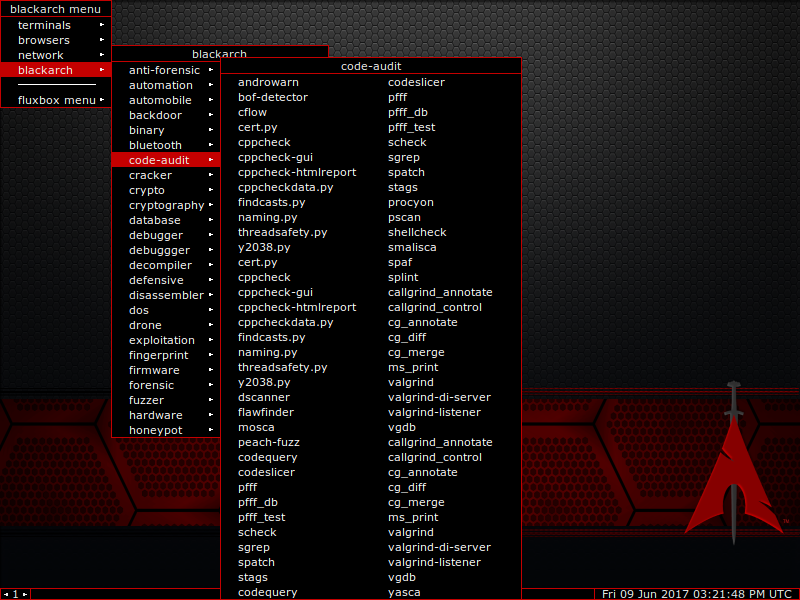
\includegraphics[width=1.0\textwidth]{Resources/Tools/BlackArch.png}
\caption{BlackArch Linux Desktop Environment}
\end{figure}

The repository currently contains 2277 tools, in the form of packages. You can install tools individually or in groups. BlackArch Linux is compatible with existing Arch installations.
\bigskip

\item[ParrotSec] is based on top of the testing branch of Debian GNU operating system. it's a Debian-based OS option that packs a lot into its programming. Developed by the team at Frozenbox's, Parrot Security is an option that's cloud-friendly \cite{parrot2019doc}.

\begin{figure}[H]
\centering
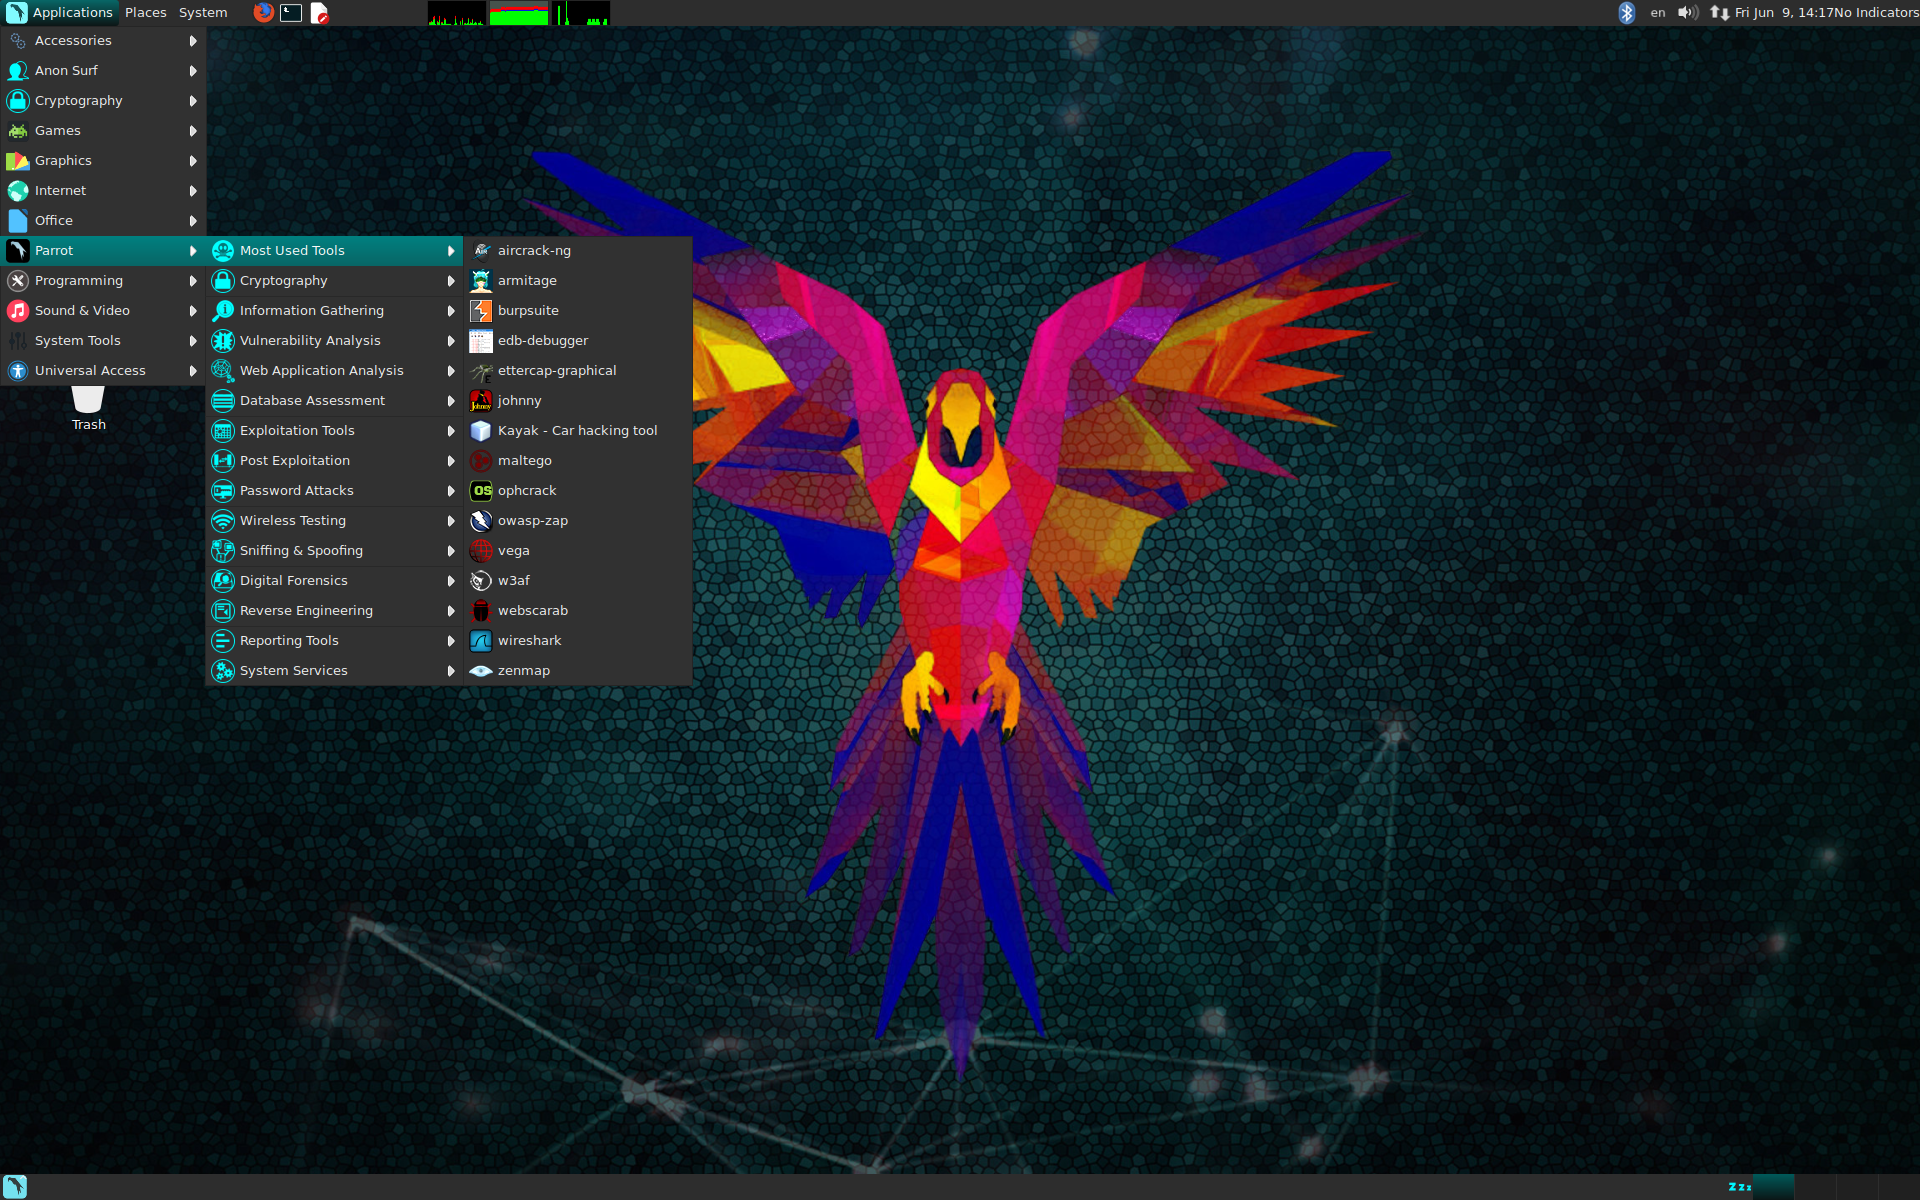
\includegraphics[width=1.0\textwidth]{Resources/Tools/Parrot.png}
\caption{Parrot Security OS Desktop Environment}
\end{figure}

The desktop environment is MATE\footnote{Visit \href{https://mate-desktop.org/}{MATE's website} for more information.}, and the default display manager is LightDM\footnote{Check \href{https://github.com/CanonicalLtd/lightdm}{LightDM's repository} online.}.The operating system is designed to specialize in ethical hacking, computer forensics, penetration testing, cryptography, and more.

\bigskip
\item[Kali Linux] is another Debian-Based Linux distribution. Developed by Offensive Security, Kali Linux is the rewrite of BackTrack. It is aimed at advanced Penetration Testing and Security Auditing. Kali contains several hundred tools which are geared towards various information security tasks, such as Penetration Testing, Security research, Computer Forensics and Reverse Engineering \cite{kali2019doc}.

\begin{figure}[H]
\centering
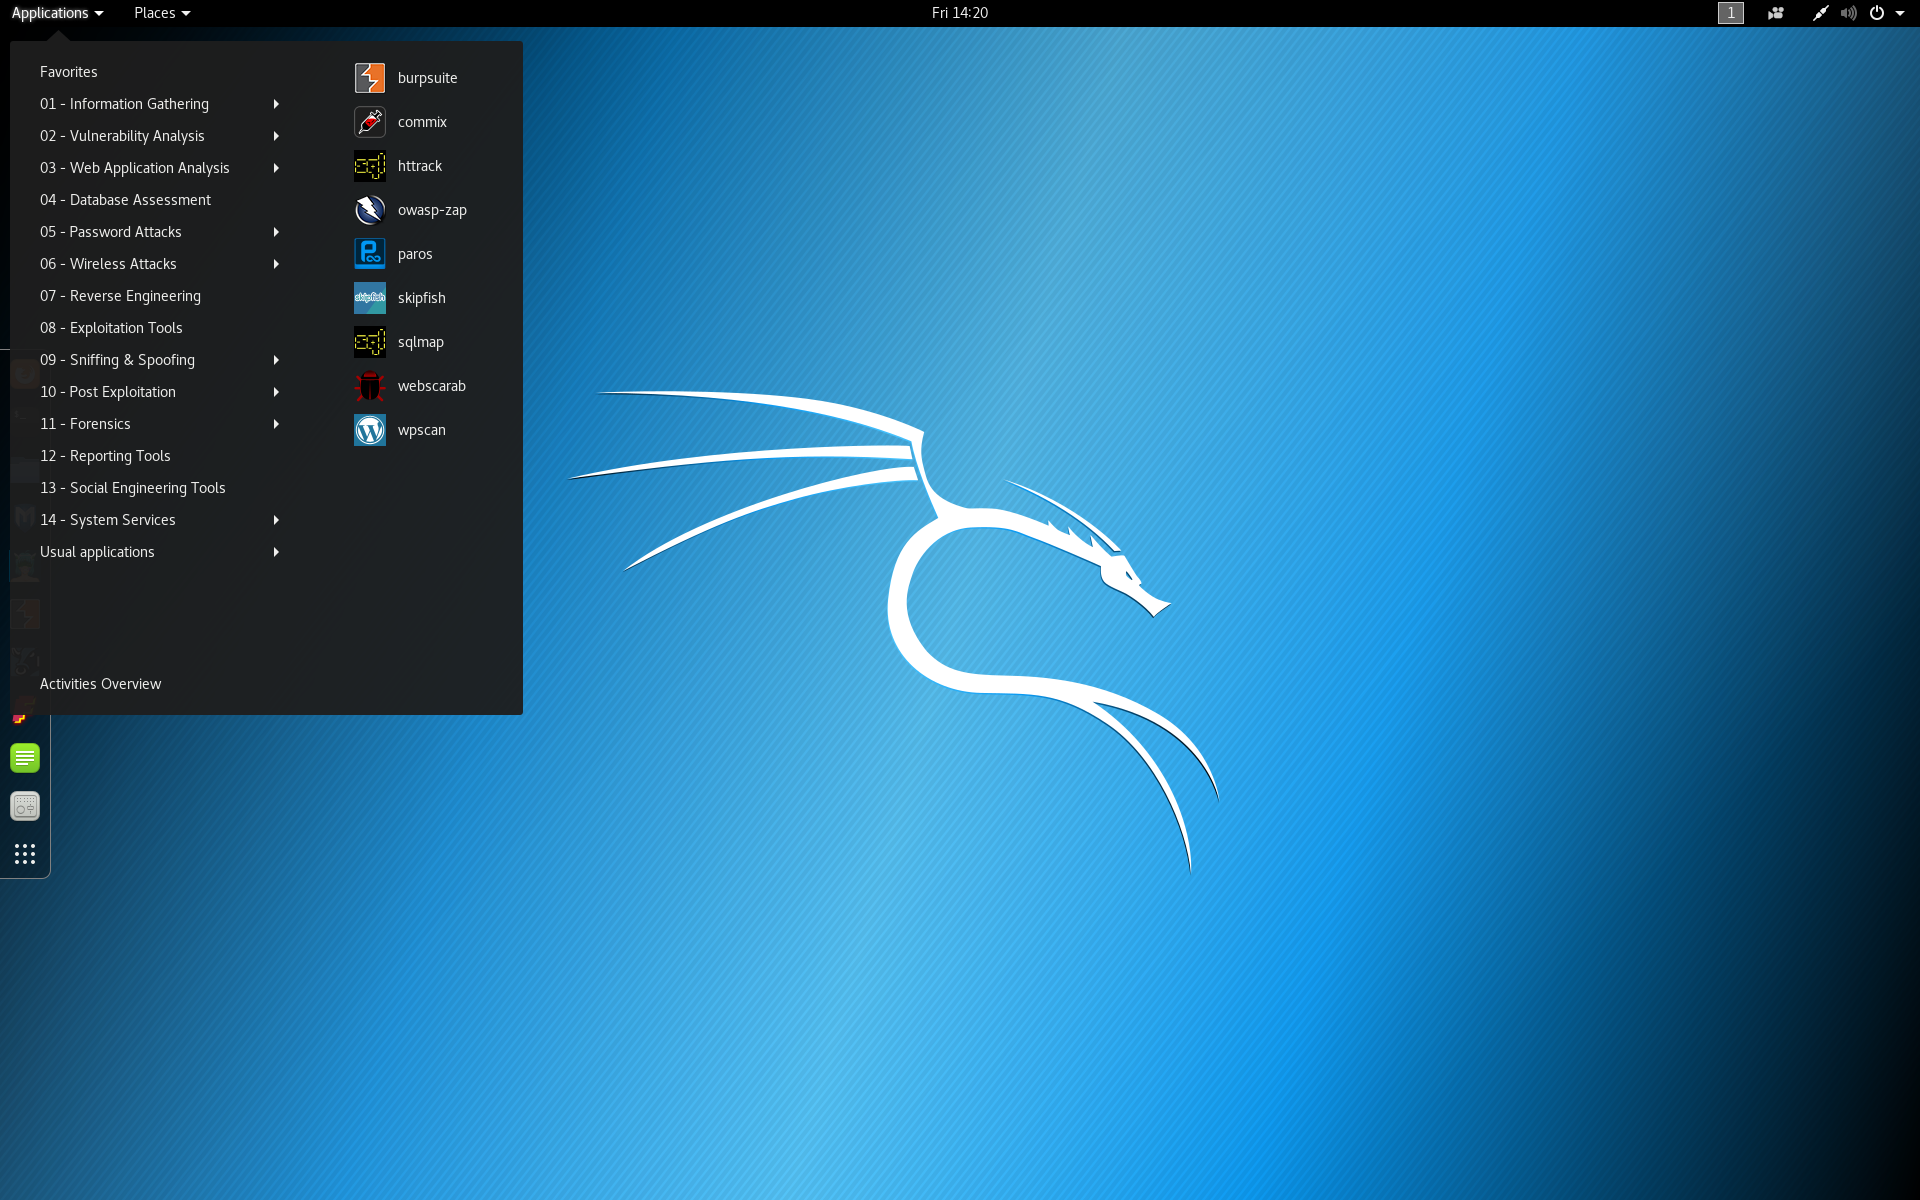
\includegraphics[width=1.0\textwidth]{Resources/Tools/Kali.png}
\caption{Kali Linux Desktop Environment}
\end{figure}

Kali Linux was released on the 13th March, 2013 as a complete, top-to-bottom rebuild of BackTrack Linux, offering the features listed below:

\begin{itemize}
    \item More than 600 penetration testing tools \cite{kali2019tools}.
    \item Open source Git tree
    \item File Hierarchy Standard (FHS) compliant
    \item ARM support\footnote{Arm CPU architecture is a set of specifications that allows developers to write software and firmware that will behave in a consistent way on all Arm-based processors. See \href{https://developer.arm.com/architectures}{ARM's website}}
\end{itemize}
\end{description}


Every operating system has its advantages and disadvantages. The tester selects the system that fits and complements his style of work and makes him feel more comfortable when using. On the other hand, a tester's tool case can vary from test to test, depending on tools' characteristics and specifications but most importantly, the identified vulnerabilities to be examined and attacked. 

\section{Database Assessment}

A database is an organized collection of data, generally stored and accessed electronically from a computer system. It is physically structured into one or more files, but to the user, the data is presented as tables containing rows and columns. A user can access data depending on his privileges.

\subsubsection{Data Handling, Storage and Transmission}
The method by which an organization's data is handled is critical to ensuring protection of sensitive information-including system architecture, security configurations, and system vulnerabilities. Organizations should ensure proper use of the database, for example:
\begin{enumerate}
\item Proper logging in order to record every action and secure transmission of data.
\item Data integrity and security.
\item Support for authorization of access and update of data.
\item Concurrent access, recovery from crashes, etc.
\end{enumerate}

\subsubsection{Defining Database and Management Systems}
Where databases are more complex they are often developed using formal design and modeling techniques. In order for data to flow as planned and the database to be managed and used properly, Management Systems come in handy. The database management system (DBMS) is the software that interacts with end users, applications, the database itself to capture and analyze the data and provides facilities to administer the database. The sum total of the database, the DBMS and the associated applications can be referred to as a "database system". Often the term "database" is also used to loosely refer to any of the DBMS, the database system or an application associated with the database. 

The types of databases that this chapter examines are all known as Database
Management Systems. These systems offer not just a data storage facility, but also tools to manage and manipulate the data stored within. These are the tools of the trade to a database administrator (DBA) or
developer, but they are equally important in a hacker toolkit.

Some recognizable DMBSs are:
\begin{itemize}
\item MySQL
\item MondoDB
\item Microsoft SQL Server
\item Oracle Database
\item PostgreSQL
\end{itemize}

\subsubsection{Testing Database Vulnerabilities}

Potential attacks on a database system can occur using the tools shown in Table \ref{Database} \cite{sqlninja2011}\cite{sqlmap2006}\cite{jsql2019}\cite{bbqsql2019}. Attacks like SQL Injection, Unauthorized privilege elevation, Denial of Service (DoS) and Exposure of backup data are some of the most common \cite{whitaker2006}.

\begin{table}[H]
\label{Database}
\centering
\begin{tabular}{c c c c}

\multicolumn{4}{c}{\textbf{\large{Database Assessment}}} \\
\hline & \small{JSQL} & \small{SqlMap} & \small{SqlNinja} \\
\hline

\small{Open-Source} & + & + & + \\ 

\small{GUI} & + && \\ 

\small{No of DBMSs Supported} & 23 & 10 & 1 \\

\small{No of Injection Techniques} & 4 & 6 & 7 \\ 

\small{Injection on Multiple Targets} & + & + &\\ 

\small{Brute-Force on sysadmin Password} & + & + & + \\ 

\small{Upload of Executables using HTTP} & + & + & + \\ 

\small{Privilege Escalation} & + & + & + \\ 

\small{Database Fingerprinting} && + & + \\ 
\hline 
 
\end{tabular}
\caption{Database Assessment tools comparison \label{DBs}}
\end{table}

\section{Information Gathering}
Preparation is crucial to any penetration test. Information gathering is the most time-consuming and laborious phase of the attack cycle but is often a major determinant of the success or failure of the engagement. 

Information Gathering software use a number of methods to discover active and responding hosts on a network, identify weaknesses, and learn how the network operates. Both passive (examination) and active (testing) techniques exist for discovering devices on a network. Passive techniques use a network sniffer to monitor network traffic and record the IP addresses of the active hosts, and can report which ports are in use and which operating systems have been discovered on the network \cite{osstmm2010}.
\subsubsection{Passive Discovery} Passive discovery can also identify the relationships between hosts-including which hosts communicate with each other, how frequently their communication occurs, and the type of traffic that is taking place-and is usually performed from a host on the internal network where it can monitor host communications. This is done without sending out a single probing packet. Passive discovery takes more time to gather information than does active discovery, and hosts that do not send or receive traffic during the monitoring period might not be reported.

\subsubsection{Active Discovery}
Active techniques send various types of network packets, such as Internet Control Message Protocol (ICMP)\footnote{The Internet Control Message Protocol (ICMP) is a supporting protocol in the Internet protocol suite. It is used by network devices, including routers, to send error messages and operational information indicating, for example, that a requested service is not available or that a host or router could not be reached.} pings, to solicit responses from network hosts, generally through the use of an automated tool. One activity, known as OS fingerprinting, enables the assessor to determine the system's OS by sending it a mix of normal, abnormal, and illegal network traffic \cite{whitaker2006}. Another activity involves sending packets to common port numbers to generate responses that indicate the ports are active. The tool analyzes the responses from these activities, and compares them with known traits of packets from specific operating systems and network services-enabling it to identify hosts, the operating systems they run, their ports, and the state of those ports. This information can be used for purposes that include gathering information on targets for penetration testing, generating topology maps, determining firewall and IDS configurations, and discovering vulnerabilities in systems and network configurations.

\subsubsection{Comparison of Techniques}
Some of the advantages of active discovery, as compared to passive discovery, are that an assessment can be conducted from a different network and usually requires little time to gather information. In passive discovery, ensuring that all hosts are captured requires traffic to hit all points, which can be time-
consuming-especially in larger enterprise networks. A disadvantage to active discovery is that it tends to generate network noise, which sometimes results in network latency. Since active discovery sends out queries to receive responses, this additional network activity could slow down traffic or cause packets to be dropped in poorly configured networks if performed at high volume. Active discovery can also trigger IDS alerts, since unlike passive discovery it reveals its origination point. The ability to successfully discover all network systems can be affected by environments with protected network segments and perimeter security devices and techniques. For
example, an environment using network address translation (NAT)-which allows organizations to have internal, non-publicly routed IP addresses that are translated to a different set of public IP addresses for external traffic-may not be accurately discovered from points external to the network or from protected segments. Personal and host-based firewalls on target devices may also block discovery traffic. Misinformation may be received as a result of trying to instigate activity from devices. Active discovery presents information from which conclusions must be drawn about settings on the target network. For both passive and active discovery, the information received is seldom completely accurate. To illustrate, only hosts that are on and connected during active discovery will be identified-if systems or a segment of the network are offline during the assessment, there is potential for a large gap in discovering devices.

\subsubsection{Tools Listing and Comparison}

A number of tools exist for use in network discovery, and it should be noted that many active discovery tools can be used for passive network sniffing and port scanning as well. Most offer a graphical user interface (GUI), and some also offer a command-line interface. Command-line interfaces may take
longer to learn than GUIs because of the number of commands and switches that specify what tests the tool should perform and which an assessor must learn to use the tool effectively. Also, developers have written a number of modules for open source tools that allow assessors to easily parse tool output. For
example, combining a tool's Extensible Markup Language (XML) output capabilities, a little scripting, and a database creates a more powerful tool that can monitor the network for unauthorized services and machines.

In the following Table, tools like: 
\begin{itemize}
\item Nmap
\item Wireshark
\item Maltego etc.
\end{itemize}
which are notable and widely used in any form of Penetration Testing, even integrated in other software, are listed and analyzed \cite{wireshark1998}\cite{nmap2019}\cite{arp2019}\cite{dmitry2019}\cite{etherape2019}.
\begin{table}[H]

\label{InfGathering}

\centering

\begin{tabular}{l c c c c c c c c}

\multicolumn{7}{c}{\textbf{\large{Information Gathering Software}}} \\
\hline & \small{arp-scan} & \small{DMitry} & \small{EtherApe} & \small{Maltego} & \small{Nmap} & \small{Wireshark} \\
\hline

\small{Open-Source} & + & + & + && + & + \\ 

\small{GUI} &&& + & + & + & + \\ 
 
\small{OS Detection} && + && + & + & + \\

\small{Port Scanning} && + &&& + &  \\ 
 
\small{Host Discovery/NAT} & + & + & + & + & + &  \\ 

\small{DNS/Whois Look-up} & + & + & + & + & + & + \\ 

\small{Data Capture} & + & + & + &  &  & + \\ 
 
\small{E-mail Search on Host} && + && + &&\\ 

\small{Export Output} & + & + & + & + & + & + \\ 
\hline
\end{tabular}
\caption{Information Gathering tools \label{Info Gathering}}
\end{table} 

Collecting information on the target system is a major part of the test since the output of those tools are highly valuable and the success of the project might depend on their results. 

\section{Sniffing and Spoofing}


Nowadays, computer networks are usually large and diverse systems that communicate using a wide variety of protocols. This complexity created the need for more sophisticated tools to monitor and troubleshoot network traffic.

Packet sniffing and spoofing are the two important concepts in network security; they are two major threats in network communication that target the lower layers of the networking infrastructure supporting applications that use the Internet. Being able to understand these two threats is essential for understanding security measures in networking.
Sniffing and Spoofing are two terms that are usually confused and often used interchangeably. The misconception that phishing/sniffing and spoofing are synonymous, based on nothing more than aesthetic similarities, pervades the Internet.

Sniffing is the use of a network interface to receive data not intended for the machine in which the interface resides. Any eavesdropping on existing traffic can be called sniffing. To be more precise, consider a LAN\footnote{A Local-Area Network (LAN) is a computer network that interconnects computers within a limited area such as a residence, school, laboratory, university campus or office building. Ethernet and Wi-Fi are the two most common technologies in use for local area networks.} having Computers A, B and C. If A and B are talking and C is trying to listen to their conversation, then C is trying a Sniffing attack provided that, according to the LAN configuration, C is not supposed to listen to conversation between A and B \cite{weidman2014}.

On the other hand, Spoofing is an active security attack in which one machine on the network masquerades as a different machine. Email spoofing is one of the best known spoofs \cite{whitaker2006}. Since core SMTP\footnote{Simple Mail Transfer Protocol (SMTP) is an Internet standard for electronic mail (email) transmission. SMTP is a connection-oriented, text-based protocol in which a mail sender communicates with a mail receiver by issuing command strings and supplying necessary data over a reliable ordered data stream channel, typically a Transmission Control Protocol (TCP) connection.} fails to offer authentication, it is simple to forge and impersonate emails \cite{harris2007}.
 
 There are many packet sniffing and spoofing tools, such as Wireshark, OWASP-Zap, WebScarab, etc. Some of these tools which widely used by security experts, as well as by attackers, can be seen in Table \ref{SniffSpoof} \cite{wireshark1998}\cite{zedattack2013}\cite{sslstrip2019}\cite{hamster2019}\cite{webscarab2019}.
\begin{table}[H]
\centering

\begin{tabular}{l c c c c c c c c c}

\multicolumn{8}{c}{\textbf{\large{Sniffing - Spoofing}}} \\

\hline & \scalebox{.65}{Etherape} & \scalebox{.65}{Hamster} & \scalebox{.65}{MITMf} & \scalebox{.65}{OWASP-Zap} & \scalebox{.65}{SSLstrip} & \scalebox{.65}{WebScarab} & \scalebox{.65}{Wireshark} \\
\hline

\scalebox{.7}{Open-Source} & + & + & + & + & + & + & + \\ 

\scalebox{.7}{GUI} & + &&& + && + & + \\ 

\scalebox{.7}{Packet Capture} & + &&& + && + & + \\ 
 
\scalebox{.7}{MITM Attack} &&& + && + && \\

\scalebox{.7}{Injections} &&& + &&&& \\ 
 
\scalebox{.7}{HTTPS to HTTP} &&& + && + &&\\ 

\scalebox{.65}{HTTP Session Hijacking} && + && + & + & + & + \\ 

\scalebox{.7}{Cookie Sniffing} && + & + &&&& + \\ 
\hline 
\end{tabular} 
\caption{Sniffing and Spoofing software \label{SniffSpoof}}
\end{table}

\section{Vulnerability Analysis/ Security Auditing}
As the number of security threats to networks and servers grows, security managers have turned to vulnerability analysis tools to identify a wide variety of potential problems on their networks. When identifying vulnerabilities, we actively search for issues that will lead to compromise in the exploitation phase. Although some security firms will just run an automated exploitation tool and hope for the best, careful study of the vulnerabilities by a skilled pentester will garner better results than any tool on its own. The tools that were examined and used in this thesis are the following:
\begin{itemize}
\item Lynis
\item Nessus
\item OpenVAS
\item Yersinia
\end{itemize}



These tools can search for misconfigured application servers, such as Web servers; and network components, such as switches and routers, that are vulnerable to known problems. They look for out-of-date applications, especially those with known problems.
\begin{table}[H]
\centering
\begin{tabular}{l c c c c c c}

\multicolumn{5}{c}{\textbf{\large{Vulnerability Analysis Tools}}} \\
\hline  & \small{Lynis} & \small{Nessus} & \small{OpenVAS} & \small{Yersinia} \\
\hline
\small{Open-Source} & + && + & + \\ 

\small{GUI} & + & + && + \\ 
 
\small{Logging} & + & + & +& + \\

\small{Plugins} && + && + \\ 

\small{Concurrent Host Scanning} & + &&& + \\ 

\small{SQL database Scan} & + & + && + \\ 

\small{Reporting} & + && + & + \\ 

\hline 

\end{tabular} 
\caption{Security Auditing for active "self"-testing \label{VulAnalysis}}
\end{table}

With new vulnerabilities being published with alarming frequency, keeping these tools current is essential.  While these tools may come with a fairly comprehensive set of tests, admins often need to create custom tests quickly and easily to examine specific conditions on their network--preferably without having to be a master programmer. For example, on our network, a common management application needed patching. We tried to write custom tests for each tool that would let us detect the unpatched application by the version number in its welcome banner.

\section{Web Application Analysis}
Web applications are complex, software-intensive systems, providing hyper-textual contents, computational facilities and services.  Furthermore, they typically work in a distributed, asynchronous fashion. Correspondingly, the quality of Web applications is a complex, multidimensional attribute.  The problem of improving the quality of Web applications involves several aspects, including the extraction of suitable models, testing, restructuring, assessment of multilingual alignment and accessibility.

Taking all those factors into consideration, the security of a Web application is crucial. Like all software, web applications may have issues when input is not properly sanitized. For example, when an application pulls data from a database based on certain user input, the application may expect specific input
such as a username and password. If, instead, the user enters special input to create additional database queries, he or she may be able to steal data from the database, bypass authentication, or even execute commands on the underlying system. Another example is when the application mismanages session related information such that the user's identity gets compromised. The information can be in the form of session cookies, passwords, secret keys etc.

To address the issue of more and more applications becoming Internet based, and the need to test the security aspects of Web applications, resources such as the open-source methodology Open Web Application Security Project (OWASP)\footnote{ For further information, see \url{https://www.owasp.org/index.php/Main_Page}} can be used and their project OWASP Top 10 2017 Project. OWASP is an open-source, community dedicated project that provides a testing framework for http-based applications. The OWASP Top 10 project is a powerful awareness document for web application security. It represents a broad consensus about the most critical security risks to web applications. According to the most recent Top 10 project, which was published in 2017, the Top 10 Web Application Security Risks are \cite{owasp2017}:
\begin{enumerate}
\item Injection
\item Broken Authentication
\item Sensitive Data Exposure
\item XML External Entities (XXE)
\item Broken Access Control
\item Security Misconfiguration
\item Cross-Site Scripting (XSS)
\item Insecure Deserialization
\item Using Components with Known Vulnernabilities
\item Insufficient Logging and Monitoring
\end{enumerate}

The tools considered in this thesis are presented in the Table \ref{WebAppAnalysis}, where some of their features are listed and compared \cite{zedattack2013}\cite{golismero2019}\cite{burp2019}\cite{webscarab2019}.
\begin{table}[H]
\centering
\begin{tabular}{l c c c c c c c}

\multicolumn{8}{c}{\textbf{\large{Web Applications Analysis Tools}}} \\

    \hline   & \scalebox{.7}{BurpSuite} & \scalebox{.7}{GoLismero} & \scalebox{.7}{Nikto} & \scalebox{.7}{OWASP-Zap} & \scalebox{.7}{Recon-ng} & \scalebox{.7}{Skipfish} & \scalebox{.7}{WebScarab}
\\
   \hline \scalebox{.8}{Open-Source} & + & + & + & + & + & + & + 
\\
   \scalebox{.8}{GUI} & + &&& + &&& +
\\
    \scalebox{.7}{Intercepting Proxy} & + && + & + & + &  & + 
\\
    \scalebox{.8}{Fuzzer} & + &&& + &&  & + 
\\
	\scalebox{.8}{(AJAX) Spider} & + &&& + & + & + & + 
\\
	\scalebox{.7}{Web Sockets (Nmap)} & + & + & + & + &&& + 
\\ 
	\scalebox{.8}{SSL Support} & + & + & + & + & + & + & + 
\\ 
	\scalebox{.7}{Automated Scans} & + &&& + && + & + 
\\ 
    \hline
\end{tabular}
\caption{Web Application and Website testing software \label{WebAppAnalysis}}
\end{table}

\section{Wireless Testing}


Wireless technologies, in their simplest sense, enable one or more devices to communicate without the need for physical connections such as network or peripheral cables. They range from simple technologies like wireless keyboards and mice to complex cell phone networks and enterprise wireless local area networks (WLAN). As the number and availability of wireless-enabled devices continues to increase, it is important for organizations to actively test and secure their enterprise wireless environments.\footnote{ For proper measures to secure IEEE 802.11-based WLANs, please refer to NIST SP 800-97, Establishing Wireless Robust
Security Networks: A Guide to IEEE 802.11i, and NIST SP 800-48 Revision 1, Guide to Securing Legacy IEEE 802.11 Wireless Networks, available at \url{http://csrc.nist.gov/publications/PubsSPs.html}.}

Although wireless networking provides great ease in setting up networked communications and offers mobility among users, it comes at a risk of security. Malicious hackers can easily detect wireless networks and gain access to your corporate network. Although a few methods are in place to enhance security, most are weak and easily broken. Wireless scans can help organizations determine corrective actions to mitigate risks posed by wireless-enabled technologies.

The wireless scanning tool should be capable of scanning all Institute of Electrical and Electronics Engineers (IEEE)\footnote{ For more information, see \url{https://www.ieee.org/}.} 802.11a/b/g/n channels, whether domestic or international. In some cases, the device should also be fitted with an external antenna to provide an additional level of radio frequency (RF) capturing capability. Support for other wireless technologies, such as Bluetooth, will help evaluate the presence of additional wireless threats and vulnerabilities. Note that devices using nonstandard technology or frequencies outside of the scanning tool's RF range will not be detected or properly recognized by the scanning tool.
Some devices also support mapping and physical location plotting through use of a mapping tool, and in some cases support Global Positioning System (GPS)-based mapping. Sophisticated wireless scanning tools allow the user to import a floor plan or map to assist in plotting the physical location of discovered devices. (It is important to note that GPS has limited capabilities indoors.)

Some of those tools are presented in Table \ref{WirelessScan} and will be used in this thesis, depending on the target system's characteristics and functions \cite{wifite2019}\cite{aircrack2019}\cite{ghost2019}\cite{kismet2019}.
 
\begin{table}[H]
\label{WirelessScan}
\centering
\begin{tabular}{l c c c c c c}

\multicolumn{6}{c}{\textbf{\large{Wireless Testing Tools}}} \\

\hline & \scalebox{.7}{aircrack-ng Suite} & \scalebox{.7}{Ghost-Phiser} & \scalebox{.7}{Kismet} & \scalebox{.7}{mdk3} & \scalebox{.7}{Wifite} \\
\hline

\small{Open-Source} & + & + & + & + & + \\ 

\small{GUI} && + & + && \\ 

\small{802.11 Traffic Capturing} & + & + & + && \\

\scalebox{.8}{Rogue Access Point Emulator} && + &&& \\ 
 
\small{ARP Poisoning} & + &&&& + \\ 

\small{WPA/WPA2 Cracking} & + &&& + & + \\ 

\small{GPS Coordinates} &&& + &&  \\ 
 
\small{Handshake Capturing} & + &&& + & + \\ 

\hline 
\end{tabular} 
\caption{Wireless Scanning and 802.11a/b/g Standard testing software \label{WirelessScan}}
\end{table}

In cases where an organization hires a contractor to implement the WLAN, it is important for the organization to conduct acceptance/verification testing to ensure that all technical system requirements are met and that the overall system is functioning effectively. The tests verify that the overall system has adequate signal coverage, performance, capacity, and security, and that management systems are in place and operating properly.

\section{Exploitation Tools and Frameworks}
This is an enthralling and challenging phase in any penetration test. Exploitation is the step where the attacker identifies potential targets for penetration attempts and selects the suitable attack methods, after analyzing the vulnerabilities. Once the targets are specified, the penetration will be performed on these targets and there will be an attempt to exploit the previously identified potential vulnerabilities.

By now, the penetration tester has acquired lots of information about the target system and network. This information is now used to break into the target system. Executing an attack is at the heart of any penetration test. If an attack is successful, the vulnerability is verified and safeguards are identified to mitigate the associated security exposure. However, at this point penetration tester should consider external factors that affect what tools to use and when. This phase acts as verification of potential vulnerabilities and thus, entails the highest risk within a penetration test so it should be performed with a lot of caution. All the possible effects need to be carefully considered; all the exploits\footnote{Exploit programs or scripts are specialized tools for exploiting specific vulnerabilities. The same cautions that apply to freeware tools apply to exploit programs and scripts.} need to
be thoroughly tested in a controlled environment before performing critical test procedures \cite{whitaker2006}.

In many cases, exploits that are executed do not grant the maximum level of potential access to an attacker \cite{erickson2008}. They may instead result in the testers learning more about the targeted network and its potential vulnerabilities, or induce a change in the state of the targeted network's security. Some exploits enable testers to escalate their privileges on the system or network to gain access to additional resources. After an initial compromise of a target system or network, the penetration tester should look for ways, to increase their access to the system. Suppose, if a penetration tester has gained a local system access, tester should make an effort to carry out further analysis on the target system to gain root privilege.
The process is represented in the loop in Figure \ref{fig:Exploit} between the attack and discovery phase in a test, thus through penetrating and exploring the target system, even more vulnerabilities and crucial information might be discovered.
\begin{figure}[H]
\centering {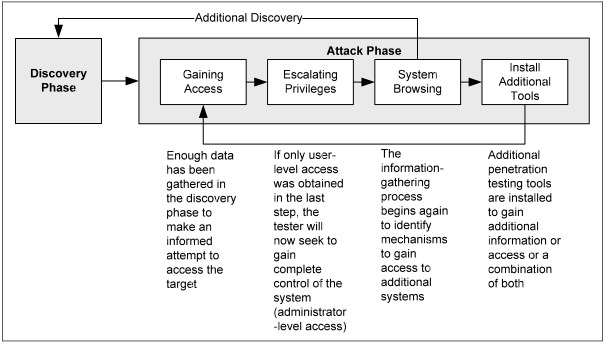
\includegraphics[scale = 0.65]{Resources/Tools/ExploitationTable.png}}
\caption{\label{fig:Exploit}Exploitation process}
\end{figure}
Most penetration testers make use of a combination of general purpose exploit applications and their own custom, scripts and applications. It should be kept into consideration that the effectiveness of any application
commercial or open source is not determined by the price tag, but the skill of the penetration tester. It is a good practice to try all possible applications and tools and decide which one work best for project environment.

In general, exploitation tools can be separated into two categories:
\begin{enumerate}
\item Tools that guide and assist the user in creating his own scripts and payloads\footnote{A payload refers to the component of a computer virus that executes a malicious activity. Apart from the speed in which a virus spreads, the threat level of a virus is calculated by the damages it causes. Viruses with more powerful payloads tend to be more harmful.}. Such type of tools are:
\begin{itemize}
\item ShellNoob \cite{shellnoob2013}
\item MSFvenom Payload Creator \cite{msfvenom2019}
\end{itemize}
\item Frameworks that provide exploits for different kind of targets and vulnerabilities. These tools can also be divided in subcategories based on where the exploit is being used on. For example, BeEF is short for The Browser Exploitation Framework \cite{beef2006}. It is a penetration testing tool that focuses on the web browser. Another example is Commix which is short for Command Injection Exploiter which is used to test web applications \cite{commix2009}. 
The most common framework in this category is Metasploit Framework with the biggest collection of exploits and payloads \cite{metasploit2004}.
\end{enumerate}

\subsubsection{Metasploit Framework}
According to SecTools.org \cite{sectools2019}, Metaslpoit Framework is the second most popular tool in the security community's favorite tools. Metasploit is the security framework originally developed in Perl by H.D. Moore in 2003 and rewritten in Ruby and acquired by Rapid7 in 2009. It is an open source project that provides the infrastructure, content, and tools to perform penetration tests and extensive security auditing. The extensible model through which payloads, encoders, no-op generators, and exploits can be integrated has made it possible to use the Metasploit Framework as an outlet for cutting-edge exploitation research. It often comes integrated in different kind of penetration testing tools and many other exploitation tools are based on it \cite{metasploit2004}. 
Key steps for exploiting a system using the Metasploit Framework can be broken
down into following steps as :
\begin{enumerate}
\item Choose and configure an exploit to be targeted.
\item Validate whether the target system is vulnerable to the chosen exploit.
\item Select and configure a payload that will be used.
\item Choose and configure the encoding schema to make sure that the payload can
evade Intrusion Detection Systems with ease.
\item Execute the exploit.
\end{enumerate}

\begin{figure}[H]
\centering {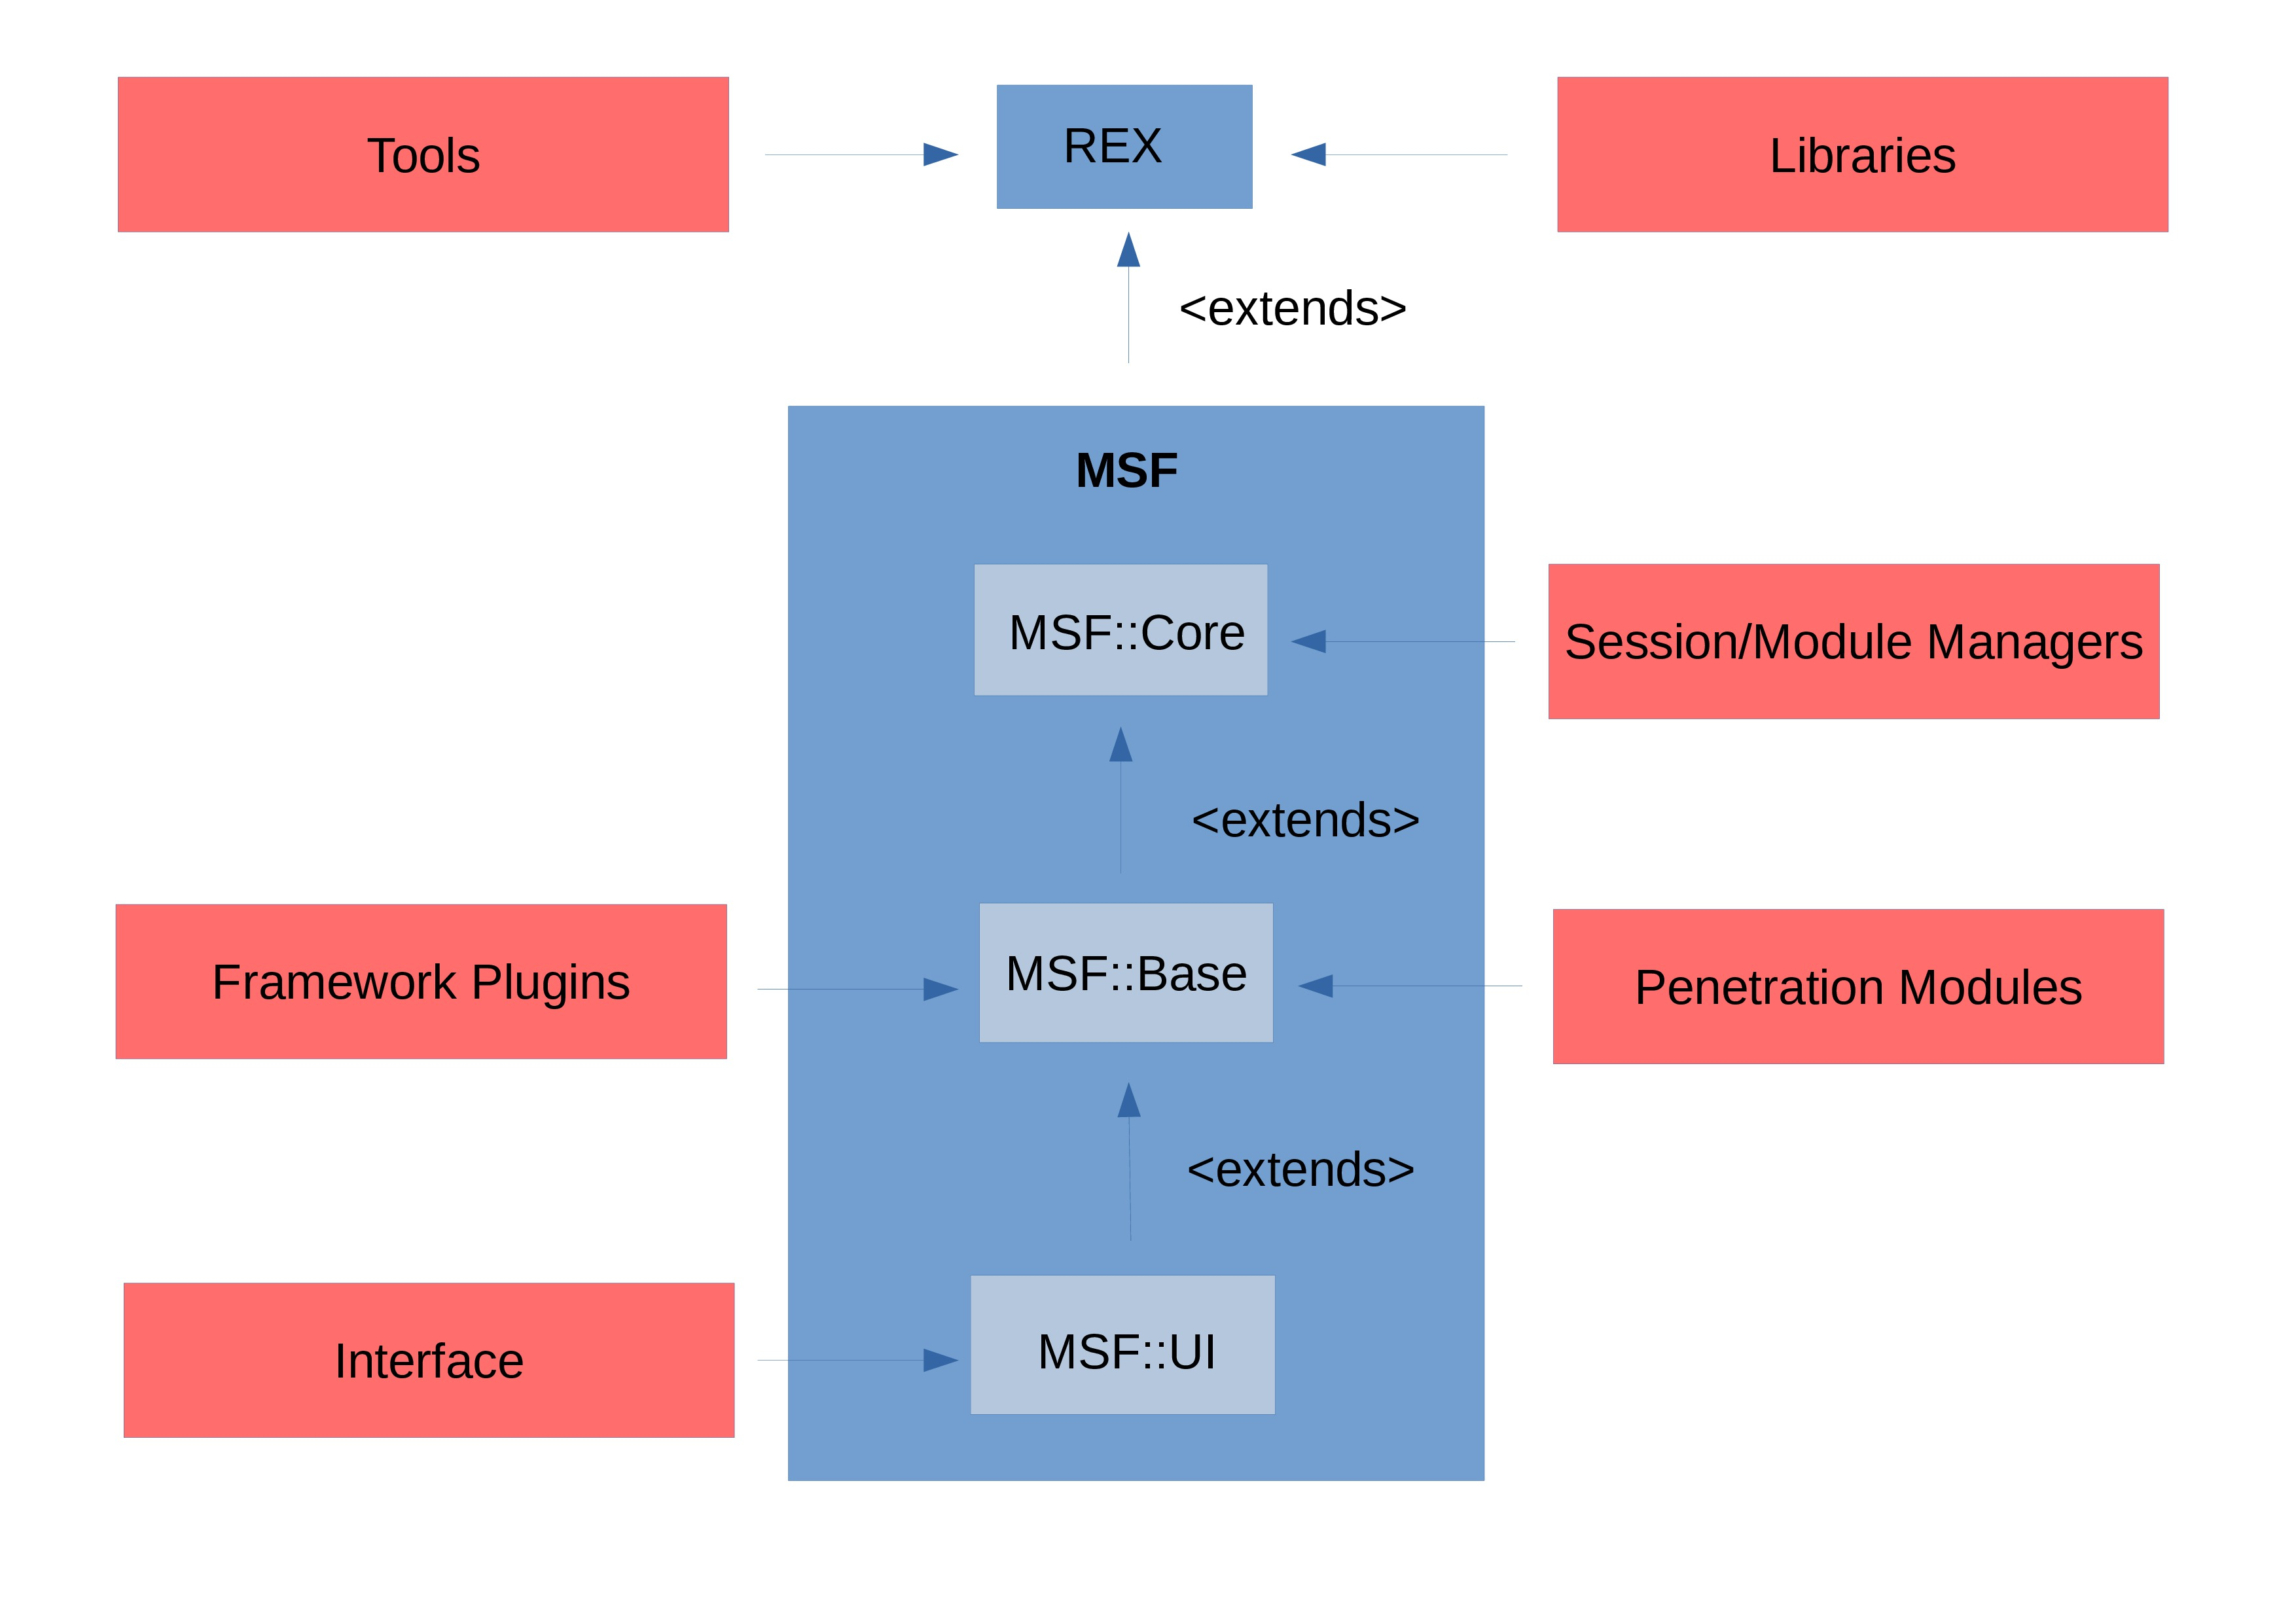
\includegraphics[scale = 0.5]{Resources/Tools/MetasploitArchitecture.jpg}}
\caption{\label{fig:Metasploit}Metasploit Framework's architecture}
\end{figure}


